\documentclass[11pt]{article}
\usepackage{geometry,marginnote} % Pour passer au format A4
\geometry{hmargin=1cm, vmargin=1cm} % 

% Page et encodage
\usepackage[T1]{fontenc} % Use 8-bit encoding that has 256 glyphs
\usepackage[english,french]{babel} % Français et anglais
\usepackage[utf8]{inputenc} 

\usepackage{lmodern,numprint}
\setlength\parindent{0pt}

% Graphiques
\usepackage{graphicx,float,grffile,units}
\usepackage{tikz,pst-eucl,pst-plot,pstricks,pst-node,pstricks-add,pst-fun,pgfplots} 

% Maths et divers
\usepackage{amsmath,amsfonts,amssymb,amsthm,verbatim}
\usepackage{multicol,enumitem,url,eurosym,gensymb,tabularx}

\DeclareUnicodeCharacter{20AC}{\euro}



% Sections
\usepackage{sectsty} % Allows customizing section commands
\allsectionsfont{\centering \normalfont\scshape}

% Tête et pied de page
\usepackage{fancyhdr} \pagestyle{fancyplain} \fancyhead{} \fancyfoot{}

\renewcommand{\headrulewidth}{0pt} % Remove header underlines
\renewcommand{\footrulewidth}{0pt} % Remove footer underlines

\newcommand{\horrule}[1]{\rule{\linewidth}{#1}} % Create horizontal rule command with 1 argument of height

\newcommand{\Pointilles}[1][3]{%
  \multido{}{#1}{\makebox[\linewidth]{\dotfill}\\[\parskip]
}}

\newtheorem{Definition}{Définition}

\usepackage{siunitx}
\sisetup{
    detect-all,
    output-decimal-marker={,},
    group-minimum-digits = 3,
    group-separator={~},
    number-unit-separator={~},
    inter-unit-product={~}
}

\setlength{\columnseprule}{1pt}

\begin{document}

\textbf{Nom, Prénom :} \hspace{8cm} \textbf{Classe :} \hspace{3cm} \textbf{Date :}\\
\vspace{-0.8cm}
\begin{center}
  \textit{La normalité est une route pavée : on y marche aisément mais les fleurs n’y poussent pas.} - \textbf{Vincent Van Gogh}
\end{center}
\vspace{-0.8cm}

\subsection*{Démonstrations}

\begin{multicols}{2}
\begin{enumerate}
  \item[1.] Démontrer le résultat de $\dfrac{2}{17} + \dfrac{3}{17}$.  \\ \Pointilles[6] \columnbreak 
  \item[2.] Démontrer le résultat de $\dfrac{2}{17} \times 3$.  \\ \Pointilles[6]
\end{enumerate} 
\end{multicols}

\subsection*{Calculer}

\begin{itemize}[label={$\bullet$}]
\item $\dfrac{6}{25} + \dfrac{10}{25} =$ \dotfill \\
\item $\dfrac{12}{32} + \dfrac{14}{32} - \dfrac{5}{32} =$ \dotfill \\
\item $\dfrac{4}{22} \times 5 + \dfrac{11}{22} =$ \dotfill \\
\item $\dfrac{7}{3} + \dfrac{3}{7} =$ \dotfill \\
\item $\dfrac{25}{12} - \dfrac{25}{12} + 20 =$ \dotfill \\
\item $4 \times \dfrac{6}{11} + \dfrac{16}{11} =$ \dotfill \\
\end{itemize} 

\subsection*{Définition}
La définition mathématique de la fraction $\dfrac{125}{254}$ est : \dotfill \\ \Pointilles[2]

\begin{multicols}{2}

\subsection*{Valeur exacte ou valeur approchée ?}
\begin{itemize}[label={$\bullet$}]
  \item $\dfrac{4}{5}$ \dotfill \\
  \item $\dfrac{120}{3}$ \dotfill \\
  \item $\dfrac{2}{3}$ \dotfill \\
  \item $\dfrac{84}{100}$ \dotfill \\
  \item $\dfrac{73}{21}$ \dotfill \\
  \item $\dfrac{137}{44}$ \dotfill \\
\end{itemize}  \columnbreak 


\subsection*{Sudoku}
\begin{figure}[H]
  \centering
  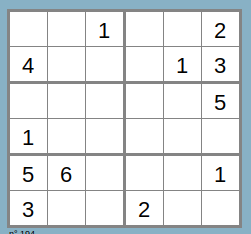
\includegraphics[width=0.8\linewidth]{6x5-fractions/sudoku-6a.png}
\end{figure}

\end{multicols}

\newpage

\textbf{Nom, Prénom :} \hspace{8cm} \textbf{Classe :} \hspace{3cm} \textbf{Date :}\\
\vspace{-0.8cm}
\begin{center}
  \textit{La normalité est une route pavée : on y marche aisément mais les fleurs n’y poussent pas.} - \textbf{Vincent Van Gogh}
\end{center}
\vspace{-0.8cm}

\subsection*{Démonstrations}

\begin{multicols}{2}
\begin{enumerate}
  \item[1.] Démontrer le résultat de $\dfrac{2}{27} + \dfrac{4}{17}$.  \\ \Pointilles[6] \columnbreak 
  \item[2.] Démontrer le résultat de $\dfrac{4}{13} \times 3$.  \\ \Pointilles[6]
\end{enumerate} 
\end{multicols}

\subsection*{Calculer}

\begin{itemize}[label={$\bullet$}]
\item $\dfrac{4}{31} + \dfrac{14}{31} =$ \dotfill \\
\item $\dfrac{12}{25} + \dfrac{6}{25} - \dfrac{5}{25} =$ \dotfill \\
\item $\dfrac{2}{22} \times 8 + \dfrac{14}{22} =$ \dotfill \\
\item $\dfrac{6}{5} + \dfrac{5}{6} =$ \dotfill \\
\item $\dfrac{23}{11} - \dfrac{23}{11} + 40 =$ \dotfill \\
\item $5 \times \dfrac{4}{17} + \dfrac{16}{17} =$ \dotfill \\
\end{itemize} 

\subsection*{Définition}
La définition mathématique de la fraction $\dfrac{125}{254}$ est : \dotfill \\ \Pointilles[2]

\begin{multicols}{2}

\subsection*{Valeur exacte ou valeur approchée ?}
\begin{itemize}[label={$\bullet$}]
  \item $\dfrac{6}{5}$ \dotfill \\
  \item $\dfrac{150}{3}$ \dotfill \\
  \item $\dfrac{3}{7}$ \dotfill \\
  \item $\dfrac{73}{100}$ \dotfill \\
  \item $\dfrac{84}{43}$ \dotfill \\
  \item $\dfrac{237}{26}$ \dotfill \\
\end{itemize}  \columnbreak 


\subsection*{Sudoku}
\begin{figure}[H]
  \centering
  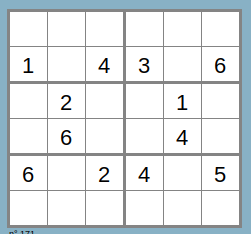
\includegraphics[width=0.8\linewidth]{6x5-fractions/sudoku-6b.png}
\end{figure}

\end{multicols}

\end{document}